\chapter{Einleitung}

Donec quam felis, ultricies nec, pellentesque eu, pretium quis, sem. Nulla consequat massa quis enim. Donec pede justo, fringilla vel, aliquet nec, vulputate eget, arcu. In enim justo, rhoncus ut, imperdiet a, venenatis vitae, justo. Nullam dictum felis eu pede mollis pretium. Integer tincidunt. Cras dapibus. Vivamus "`elementum semper nisi"' \cite{Fischer.2010b}. Aenean vulputate eleifend tellus. Aenean leo ligula, porttitor eu, consequat vitae, eleifend ac, enim. Aliquam lorem ante, dapibus in, viverra quis, feugiat a, tellus. Phasellus viverra nulla ut metus varius laoreet. Quisque rutrum. Aenean imperdiet. Etiam ultricies nisi vel augue. Curabitur ullamcorper ultricies nisi. 


\section{Forschungsfragen}
Vestibulum fringilla pede sit amet augue. In turpis. Pellentesque posuere. Praesent turpis. Aenean posuere, tortor sed cursus feugiat, nunc augue blandit nunc, eu sollicitudin urna dolor sagittis lacus \cite[S. 33-39]{Brambilla.2012}. Donec elit libero, sodales nec, volutpat a, suscipit non, turpis. Nullam sagittis. Suspendisse pulvinar, augue ac venenatis condimentum, sem libero volutpat nibh, nec pellentesque velit pede quis nunc. Vestibulum ante ipsum primis in faucibus orci luctus et ultrices posuere cubilia Curae; Fusce id purus. Ut varius tincidunt libero. Phasellus dolor.  
\begin{figure}
	\centering
		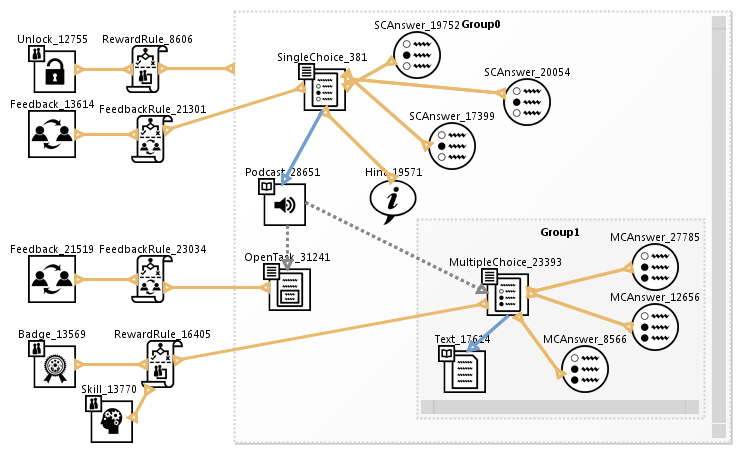
\includegraphics[width=0.7\textwidth]{Bilder/emendo.png}
	\caption{Beispiel 1 zum Einfügen einer Grafik}
	\label{fig:bsp1}
\end{figure}

In ac felis quis tortor malesuada pretium. Pellentesque auctor neque nec urna. Proin sapien ipsum, porta a, auctor quis, euismod ut, mi. Aenean viverra rhoncus pede. Pellentesque habitant morbi tristique senectus et netus et malesuada fames ac turpis egestas \cite{LohrRichter.1993}. Ut non enim eleifend felis pretium feugiat. Vivamus quis mi. Phasellus a est. Phasellus magna. In hac habitasse platea dictumst. Curabitur at lacus ac velit ornare lobortis. Curabitur a felis in nunc fringilla tristique. 

\section{Ziel der Arbeit}

Vestibulum fringilla pede sit amet augue. In turpis. Pellentesque posuere. Praesent turpis. Aenean posuere, tortor sed cursus feugiat, nunc augue blandit nunc, eu sollicitudin urna dolor sagittis lacus \cite{Lammel.2012}. Donec elit libero, sodales nec, volutpat a, suscipit non, turpis. Nullam sagittis. Suspendisse pulvinar, augue ac venenatis condimentum, sem libero volutpat nibh, nec pellentesque velit pede quis nunc. Vestibulum ante ipsum primis in faucibus orci luctus et ultrices posuere cubilia Curae; Fusce id purus. Ut varius tincidunt libero. Phasellus dolor. Maecenas vestibulum mollis diam. Pellentesque ut neque. Pellentesque habitant morbi tristique senectus et netus et malesuada fames ac turpis egestas. In dui magna, posuere eget, vestibulum et, tempor auctor, justo \cite{Kelly.2008}. In ac felis quis tortor malesuada pretium. 

\begin{table} [ht]
\centering
	\begin{tabular}{rcccrr}
		\toprule
		\multicolumn{1}{l}{Anzahl}&
		\multicolumn{2}{c}{rel. Fehler (\%)}&&
		\multicolumn{2}{c}{abs. Fehler}\\
		\cmidrule{2-3}
		\cmidrule{5-6}
		& mittl. & max. && mittl. & max. \\
		\midrule
		$<$ 1000      & 3,8 & 5,2 && 38 & 52\\
		1000 -- 5000  & 4,2 & 7,9 && 840 & 1580\\
		5000 -- 10000 & 2,7 & 3,5 && 433 & 1350\\
		$>$ 10000     & 0,9 & 1,2 && 11 & 321\\
		\bottomrule
	\end{tabular}
	\caption[Hier steht die TabellenCaption]{Fehlerhäufigkeiten in Abhängigkeit zur Anzahl - Tabellenbeispiel}
	\label{tab:Auswertungskategorien}
\end{table}

Pellentesque auctor neque nec urna. Proin sapien ipsum, porta a, auctor quis, euismod ut, mi. Aenean viverra rhoncus pede. Pellentesque habitant morbi tristique senectus et netus et malesuada fames ac turpis egestas (siehe \ref{tab:Auswertungskategorien}). Ut non enim eleifend felis pretium feugiat. Vivamus quis mi. Phasellus a est. Phasellus magna. In hac habitasse platea dictumst. Curabitur at lacus ac velit ornare lobortis. Curabitur a felis in nunc fringilla tristique.

\section{Struktur der Arbeit}

Vestibulum fringilla pede sit amet augue. In turpis. Pellentesque posuere. Praesent turpis. Aenean posuere, tortor sed cursus feugiat, nunc augue blandit nunc, eu sollicitudin urna dolor sagittis lacus. Donec elit libero, sodales nec, volutpat a, suscipit non, turpis. Nullam sagittis. Suspendisse pulvinar, augue ac venenatis condimentum, sem libero volutpat nibh, nec pellentesque velit pede quis nunc. Vestibulum ante ipsum primis in faucibus orci luctus et ultrices posuere cubilia Curae; Fusce id purus. Ut varius tincidunt libero. Phasellus dolor.

